%% =====================================================================
%% Results / Scaling across datasets -- owner: Harshaan.
%% Measurements only; interpretation in sec/harshaan/disc-scaling.tex.
%% Sources: fig/table_pipeline.tex, fig/table_perrank.tex, Table tab:human;
%% human per-pair task times from PGA_PAIR_TASKS (jobs 61277457, 61277456);
%% primates14 largest task from docs/agent/decision-gate-2.md (earlier build,
%% same alignment code). Figure: fig/make_scaling_fig.py.
%% =====================================================================

\subsection{Scaling across datasets}\label{sec:results:scaling}

Fig.~\ref{fig:scaling} compares the four datasets. At the largest doubling
of ranks tested for each, the total time falls by 1.78$\times$ on yeast7
(4 to 8 ranks), 1.41$\times$ on primates4.chr6 (8 to 16), 0.99$\times$ on
primates14.chr6 (32 to 64) and 1.62$\times$ on hsapiens90.chr6 (32 to 64).
At its largest rank count, the slowest rank's alignment time is 1.70 times
the average on primates4.chr6, 6.59 on primates14.chr6 and 1.49 on
hsapiens90.chr6.

On hsapiens90.chr6, the per-pair records sum to 6,013\,s of alignment work
at 32 ranks and 6,426\,s at 64, and the most expensive contig pair, a
self-alignment, takes 34\,s, about 0.5\% of the total. On primates14.chr6
the most expensive pair takes 773\,s, about 7\% of all alignment work
(measured with an earlier build that runs the same alignment code). From 32
to 64 ranks on hsapiens90.chr6, the alignment stage falls from 252.20\,s to
151.92\,s, while the average rank's alignment time falls from 187.12\,s to
100.47\,s; the sort falls from 22.65\,s to 18.16\,s. Peak memory per rank
falls from 22.9\,GB to 14.1\,GB, and memory summed over ranks rises from
675\,GB to 747\,GB.

\begin{figure}[h]
\centering
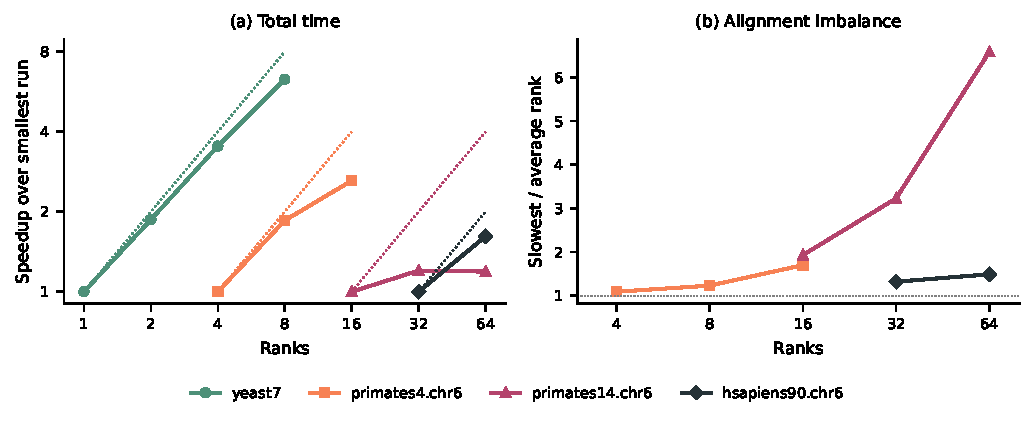
\includegraphics[width=\textwidth]{fig/scaling_summary.pdf}
\caption{Scaling across the four datasets. (a) Speedup of the total time
over each dataset's smallest run; dotted lines show ideal scaling.
(b) Slowest rank's alignment time divided by the average
(Table~\ref{tab:perrank} and Section~\ref{sec:results:human}).}\label{fig:scaling}
\par\noindent Alt text: Two line plots against ranks. Yeast7 and the human
dataset stay close to ideal speedup, primates4.chr6 falls below it, and
primates14.chr6 stops improving after 32 ranks. Alignment imbalance rises
to 6.6 on primates14.chr6 at 64 ranks but stays below 1.5 on the human
dataset.
\end{figure}
